\chapter{Perfilado de Señal WiFi}


\section{Simulación}
\begin{figure}[!htb]
	\centering
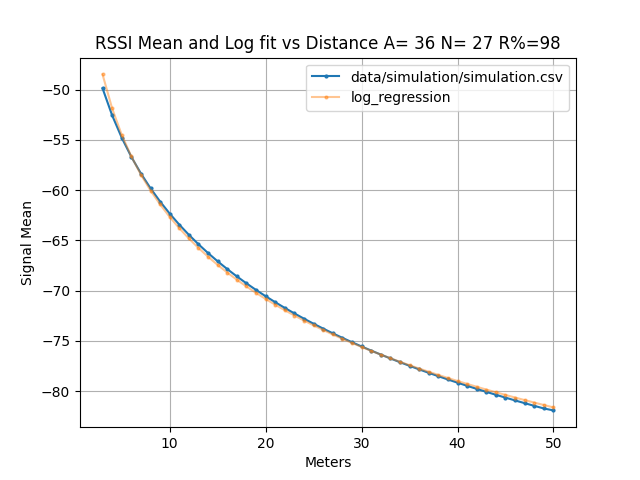
\includegraphics[width=0.8\textwidth]{Figuras/profiling/simulation/simulation_mean_fit.png}
	\captionsetup{margin=2cm}
 	\caption[Media de RSSI segregado por distancia de la medición vs regresión logarítmica, simulación usando NS3.]{Media de RSSI segregado por distancia de la medición vs regresión logarítmica, simulación usando NS3.}
	\label{fig:profiling-result-sim}
\end{figure}


Para poder saber la relación entre los \textbf{RSSI} recibidos y la distancia es necesario perfilar nuestro dispositivo. Esto se debe a que distintos dispositivos \textbf{Wi-Fi} con distinto hardware tienen distintas características de transmisión y recepción, por ejemplo: por la antena misma que este posee. Al perfilar entonces sabremos con qué intensidad recibe la señal transmitida por el dispositivo móvil de prueba y cómo decae esa señal a medida que este se aleja. Esto tiene como objetivo final averiguar los valores de N y A para completar nuestra fórmula de conversión de \textbf{RSSI} a distancia.

El perfilado se realizó primero en un ambiente simulado para probar la eficacia de nuestros algoritmos y finalmente un experimento real.
Como se describió anteriormente en la sección de infraestructura de simulación se uso \textit{NS3} configurado como una red \textbf{ADHOC}. En este experimento en particular se les aplico a los nodos un modelo de movilidad donde un nodo \textbf{Sniffer} permanece quieto mientras que el otro el nodo \textbf{Objetivo} se aleja de este hasta \textbf{100} metros y su señal decae.

Después de llevar a cabo la simulación y recopilar los datos resultantes en un archivo .csv, procedimos con el análisis de los mismos. Los datos recogidos representaban la relación entre la intensidad de la señal \textbf{RSSI} y la distancia entre los nodos, que fue crucial para perfilar nuestro dispositivo.

El gráfico generado a partir de estos datos muestra cómo la señal \textbf{RSSI} decae a medida que la distancia entre el nodo \textbf{Objetivo} y el nodo \textbf{Sniffer} aumenta, como se puede observar en la Figura \ref{fig:profiling-result-sim}.

En la gráfica, se puede apreciar un decaimiento de la señal del nodo \textbf{Objetivo} conforme este se aleja del nodo \textbf{Sniffer}. Se observa un rango efectivo de menos de \textbf{100} metros, con pérdidas señal frecuentes alrededor de los \textbf{51} metros.

Este experimento nos proporcionó valores preliminares de \textbf{N} y \textbf{A}, necesarios para nuestra fórmula de conversión de \textbf{RSSI} a distancia, validando así la efectividad de nuestros algoritmos en un entorno simulado. Este perfilado constituye un paso crucial antes de proceder a experimentos en entornos reales.

Se puede observar una pequeña deriva entre la ubicación real y la predicha, esto se debe a que el \textit{fitting} de la curva simulada no es perfecto y tuvo un pequeño margen de error. Ese error depende de la distancia de la medición ya que hay partes de la curva que se ajustan mejor que otras, en este caso cuanto mas cerca a los nodos el ajuste es peor.

A pesar de ser un entorno controlado, estos resultados nos proporcionan una visión preliminar útil de cómo se comportaría nuestro sistema en la realidad. Los próximos pasos implicarán la realización de pruebas en entornos reales para validar y afinar aún más nuestros parámetros y algoritmos.

\section{Experimento Preliminar de Perfilado Con \textbf{“\textit{steps}”} }


%\begin{figure}[!htb]
%	\centering
%	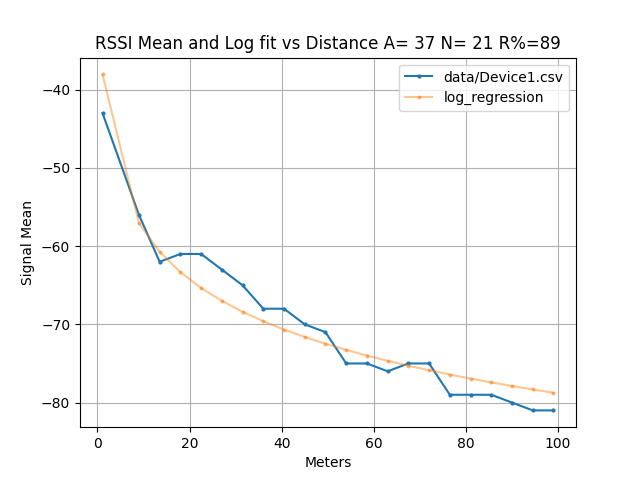
\includegraphics[width=0.8\textwidth]{Figuras/profiling/device1/device1_regression.png}
%	\captionsetup{margin=2cm}
%	\caption[Media de RSSI segregado por distancia de la medición vs regresión logarítmica, prueba de campo]{Media de RSSI segregado por distancia de la medición vs regresión logarítmica, prueba de campo con \textit{steps}”, con ESP8266 en campo de deportes UNGS. Se hallaron valores para \textbf{A=37}, \textbf{N=21} y \textbf{R(residual)=89\ }}
%	\label{fig:dev1-regression}
%\end{figure}


Llevamos a cabo una serie de experimentos en el campo de deportes de la UNGS, donde los \textbf{ESP8266} capturaban datos de señal, que luego eran procesados por una \textbf{RPI}. Estos datos eran agrupados por distancia y, a través de la recopilación de 21 mediciones para cada dispositivo, con 200 muestras en cada una, pudimos obtener una visión detallada del comportamiento de la señal.

La figura \ref{fig:dev2-dev1-regression} muestra los resultados obtenidos de este experimento en el mundo real. En el eje X se puede observar la distancia real desde el dispositivo \textbf{ESP8266} hasta el dispositivo móvil transmisor en metros, mientras que en el eje Y se representa el \textit{RSSI} medido. Cada punto en el gráfico representa una medición individual del \textit{RSSI} en una determinada distancia.



Puede observarse que a medida que la distancia aumenta, el \textit{RSSI} disminuye de manera bastante consistente, lo que se alinea con lo que esperaríamos de la pérdida de señal en función de la distancia en un entorno con mínima interferencia. Sin embargo, también se pueden identificar algunas variaciones y anomalías en los datos, posiblemente debido a factores ambientales no controlados o a variaciones inherentes en la recepción de la señal.
\begin{center}
	\centering
	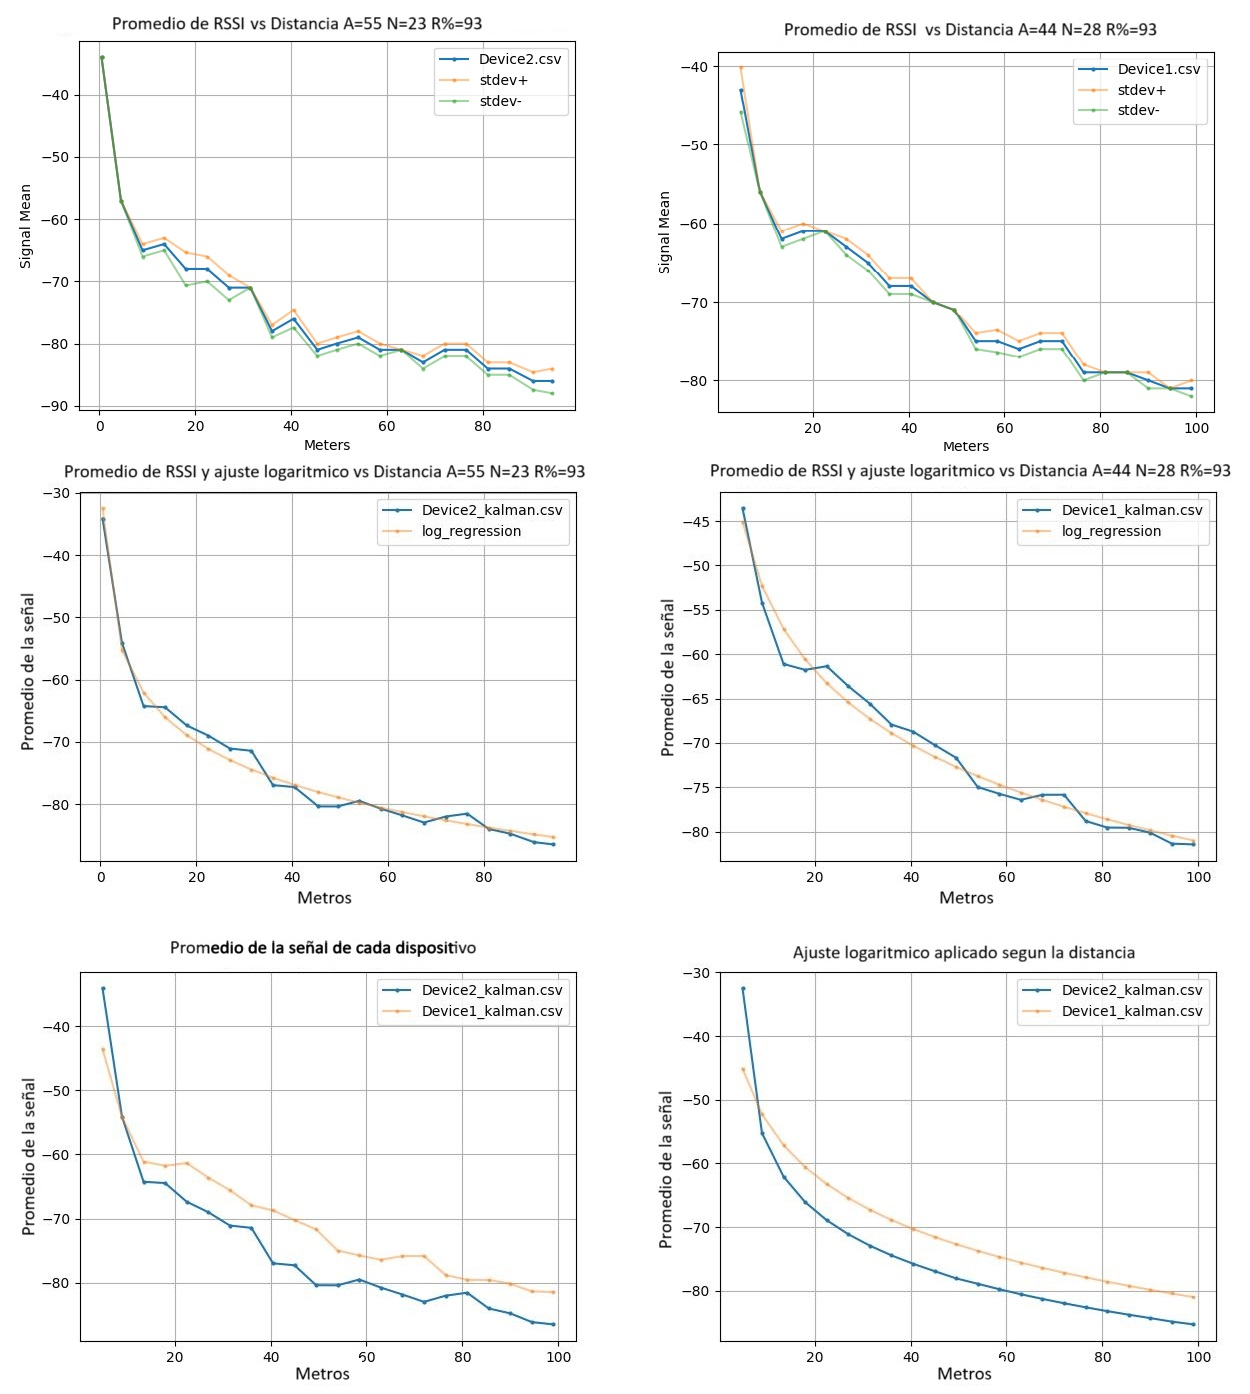
\includegraphics[width=1\textwidth]{Figuras/profiling/preliminar-experiment.jpg}
	\captionsetup{margin=2cm}
	\caption[Media de RSSI segregado por distancia de la medición vs regresión logarítmica, prueba de campo]{Media de RSSI segregado por distancia de la medición vs regresión logarítmica, prueba de campo con \textit{steps}”, con ESP8266 en campo de deportes UNGS. Se hallaron valores del dispotivo 1 para \textbf{A=37}, \textbf{N=21} y \textbf{R(residual)=89}
    Para el dispositivo 2 \textbf{A=49}, \textbf{N=18} y \textbf{R(residual)=88 }
 }
\label{fig:dev2-dev1-regression}
\end{center}
Finalmente, realizamos una regresión logarítmica para obtener una representación ajustada de la relación entre la distancia y el \textit{RSSI}. El resultado de esta regresión nos proporcionó los parámetros \textbf{A} y \textbf{N}, que luego se utilizarían en la siguiente fase de nuestro estudio para implementar la multilateración.

\section{Experimento de campo de Perfilado sin \textbf{“\textit{steps}”} }

El perfilado sin \textit{steps} nos permitió realizar el experimento mas rápidamente. Para hallar los valores de N y A en distintos ambientes con facilidad y para múltiples nodos a la vez sin necesidad de estar enchufado por cable o tomar nota manualmente de a que distancia uno se encuentra e interrumpir mediciones entre cada distancia. Esto permitió completar una medición en 15 minutos en vez de 1 hora. Además se presenta como una opción ideal al reinstalar nodos en una nueva ubicación.

Se encontró que si bien existían diferencias entre nodos eso no era lo que mas preocupaba sino que también ciertos nodos presentaban interferencias muy grandes. Esto nos lleva a pensar en desperfectos en dichos nodos o interferencia en el área del experimento que afecto a algunos nodos si y a otros no.

Este experimento se realizo en el campus de la UNGS a diferencia del experimento inicial que se realizo en el campo de deportes.

Se colocaron múltiples nodos en una linea perpendicular al recorrido y se procedió a alejarse hasta llegar a los 30 metros. Finalmente una vez completado el recorrido se espero a que los nodos completen su captura y descarguen los datos. 





